\documentclass[useAMS,usenatbib,usegraphicx]{mn2e} 
%=========================================================================
\usepackage{amsmath} 
\usepackage{amssymb} 
\usepackage{graphicx}
\usepackage{grffile}
\usepackage[dvips]{epsfig}
\usepackage{epsfig}  
\usepackage{color}
\usepackage{hyperref}
\newcommand{\apj}{ApJ}  
\newcommand{\jcap}{JCAP}  
\newcommand{\apjs}{ApJS}  
\newcommand{\pasa}{PASA}  
\newcommand{\apjl}{ApJL}  
\newcommand{\aj}{AJ}  
\newcommand{\mnras}{MNRAS}  
\newcommand{\mnrassub}{MNRAS accepted}  
\newcommand{\aap}{A\&A}  
\newcommand{\aaps}{A\&AS}  
\newcommand{\araa}{ARA\&A}  
\newcommand{\nat}{Nature}  
\newcommand{\physrep}{PhR}
\newcommand{\pasp}{PASP}    
\newcommand{\pasj}{PASJ}    
\newcommand{\hMpc}{{\ifmmode{h^{-1}{\rm Mpc}}\else{$h^{-1}$Mpc}\fi}}  
\newcommand{\Mpc}{{\ifmmode{{\rm Mpc}}\else{Mpc}\fi}}  
\newcommand{\hMsun}{{\ifmmode{h^{-1}{\rm{M_{\odot}}}}\else{$h^{-1}{\rm{M_{\odot}}}$}\fi}}
\newcommand{\Msun}{{\ifmmode{{\rm{M_{\odot}}}}\else{${\rm{M_{\odot}}}$}\fi}}
\newcommand{\kms}{{\ifmmode{{\rm{km\ s}^{-1}}}\else{km $\rm{s}^{-1}$}\fi}}


\begin{document}

%=========================================================================
%		FRONT MATTER
%=========================================================================
\title[LG satellite alignments]{Satellite Alignments in the Local Group}
\author[J.E. Forero-Romero \& V. Arias]
{Jaime E. Forero-Romero $^{1}$ \thanks{je.forero@uniandes.edu.co},
Ver\'onica Arias$^1$\\
%%
$^1$ Departamento de F\'isica, Universidad de los Andes, Cra. 1
  No. 18A-10 Edificio Ip, CP 111711, Bogot\'a, Colombia \\
}

\maketitle

\begin{abstract}
We focus on the spatial distribution of bright ($M_V<-8$) satellites and
pairs of galaxies with similar masses, isolation and kinematic
configurations as the Local Group. 
\end{abstract}

\begin{keywords}Galaxies: halos --- Galaxies: high-redshift --- Galaxies: statistics
--- Dark Matter --- Methods: numerical 
\end{keywords}

\section{Introduction}

\section{Local Group Analogues in the Illustris Simulation}
\label{sec:NumericalSetup}

We use publicly available data from the Illustris Project 
\citep{2014MNRAS.444.1518V}. 
This suite of cosmological simulations, performed using the quasi-Lagrangian
code AREPO \citep{2010MNRAS.401..791S}, follow the coupled evolution of dark 
matter and gas and includes parametrizations to account for the effects of
gas cooling, photoionization, star formation, stellar feedback, black
hole and super massive black hole feedback. 

The simulation volume is a cubic box of $75$ \hMpc\ on a side.
The cosmological parameters correspond to a $\Lambda$CDM cosmology
consistent with WMAP-9 measurements \citep{2013ApJS..208...19H}. 

We extract halo and galaxy information from the Illustris-1 simulation
which has the highest resolution in the current release of the
Illustris Project.
Illustris-1 has $1820^3$ dark matter particles and $1820^3$ initial gas
volumen elements. 
This corresponds to a dark matter particle mass of
$6.3\times 10^6$\Msun\ and a minimum mass for the baryonic volume
element of $8.0\times 10^7$\Msun. 
The corresponding spatial resolution is $1.4$ kpc for the dark matter
gravitational softening and $0.7$ kpc for the typical size of the
smallest gas cell size. 

We compute the cosmic web from the DM information in the
Illustris-3 simulation which share the same structure information with
Illustris-1 on scales of $1$ \Mpc.  
Illustris-3 has $455^3$ DM particles, corresponding to
$4.0\times 10^8$ \Msun in DM particle mass and $5.7$ kpc for the DM
gravitational softwning lentgh.
 

\subsection{Sample Selection: Local Group Analogues}

We build two samples of galaxy pairs. 
The first is a general sample of isolated pairs (IP) and the
second sample correspond to Local Group pairs (LGP).
The halos in these samples only include the DM halos with maximum
circular velocities in the range $ 150\ \kms <V_{\rm max}< 350\ \kms$. We
exclude sub-halos from this selection. 

From this set of DM halos we construct the IP sample as follows.
For each halo $A$ we find its closest halo $B$, if halo $A$ is also
the closest to halo $B$, the two halos are considered as a pair. 
Another way to phrase this selection is that pairs do not have
neighbors closer than the pair's distance.
We exclude the pairs that have overlapping virial radii. 
We use this information to exclude all the pairs that have separations
smaller than the sum of their virial radii, i.e. we exclude
We find $49$ pairs with those conditions.

We then count the number of galaxies with $M_V<-9$ inside the virial
radius of each halo, including the central galaxy.
We only keep pairs where both halos have at least 5 bright galaxies, 
reducing the sample to $24$ pairs.  
This is the IP sample.

We build the LGP sample by keeping the pairs in the IP sample with
a separation between its brightest galaxies of $0.75\ \Mpc <R_{AB}< 1.50\ \Mpc$
and a negative relative radial velocity (including the Hubble flow) 
These intervals are close to the Local Group observed values.
The LGP sample is reduced to $12$ pairs.

Figure \ref{fig:samples} show the results for the IP and LGP samples
in the plane of radial velocity versus distance.

\begin{figure}
\centering
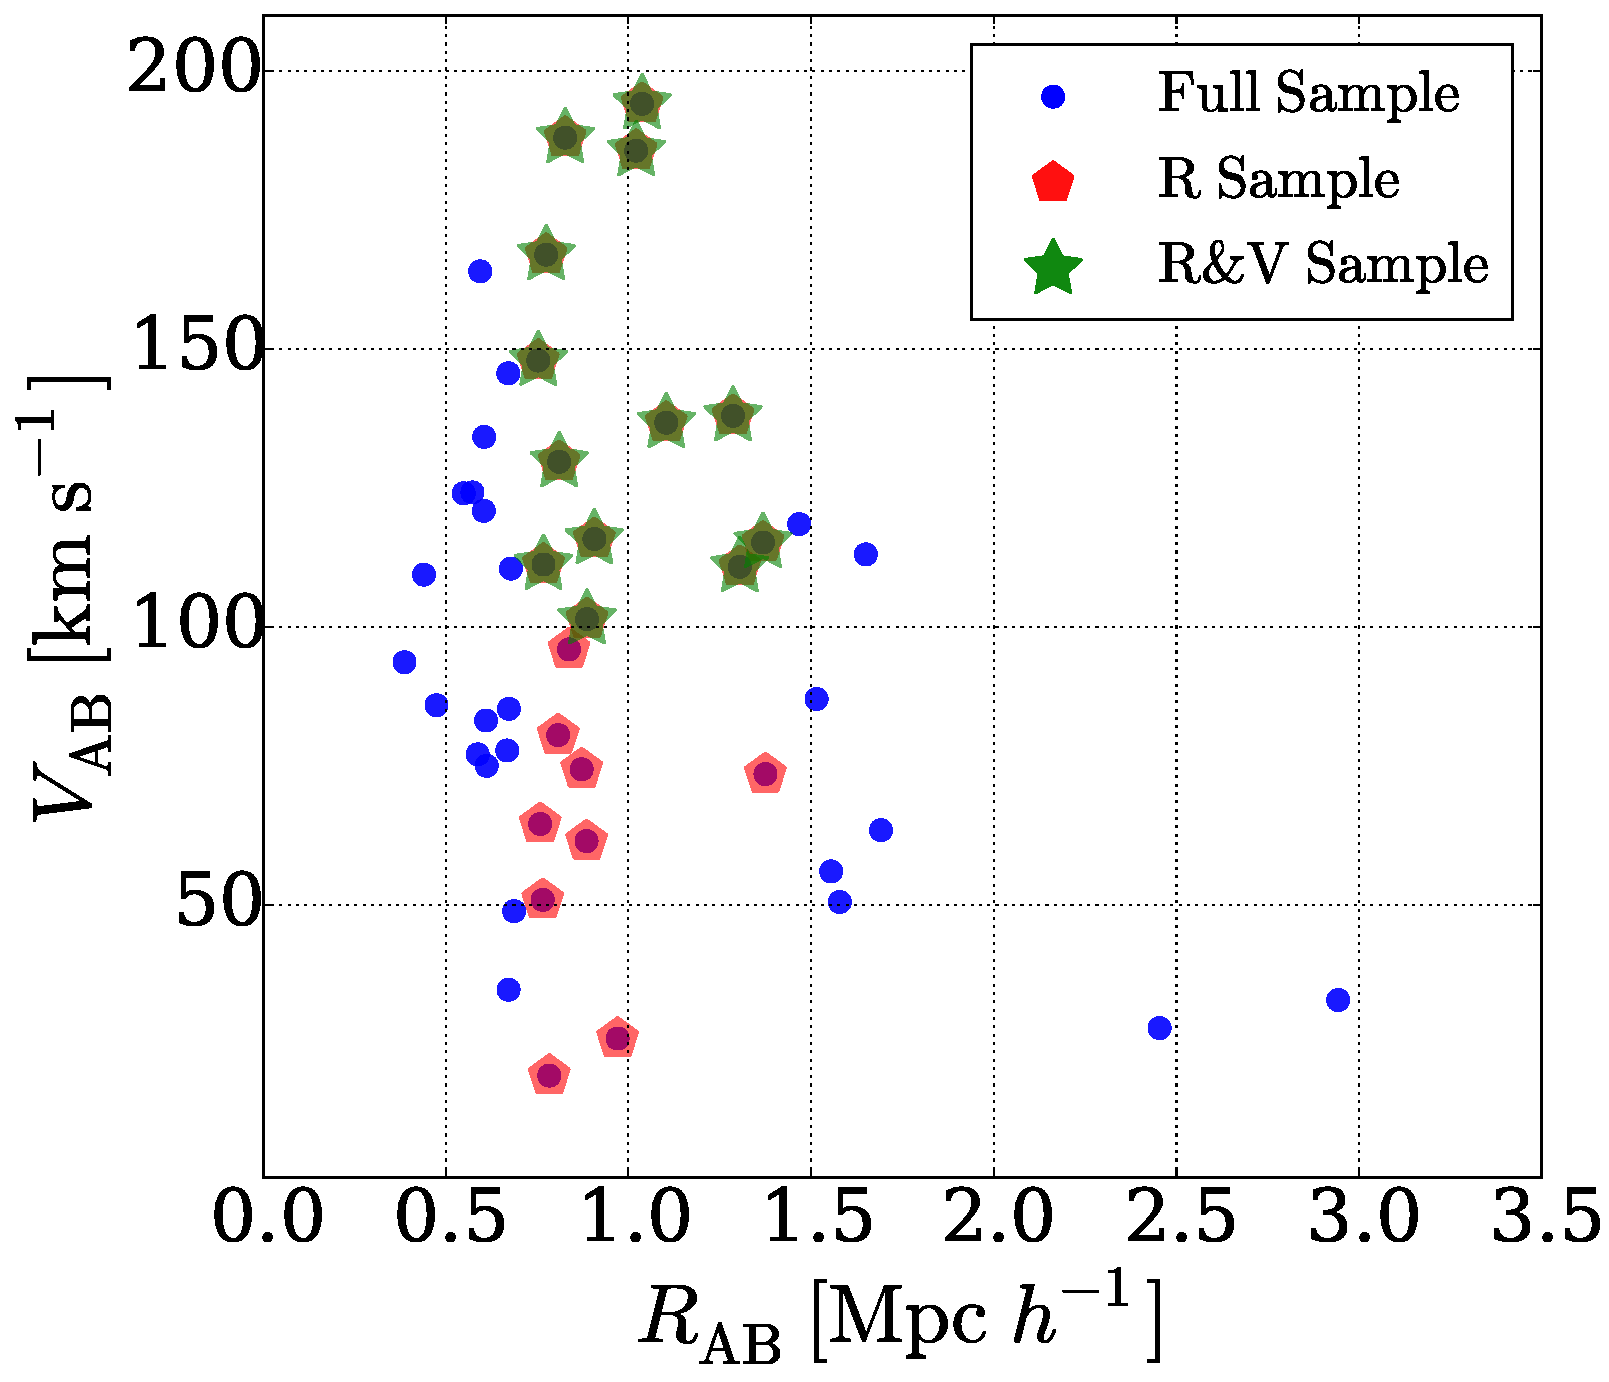
\includegraphics[width=0.5\textwidth]{v_r_pairs.pdf}
\caption{Halo pair samples used in this paper located in the
  plane of relative radial velocity $V_{r,AB}$ versus 
  distance $R_{AB}$ between the two halos in the pair.
  The IP sample (24 pairs) is a general pair sample, while the LGP
  sample (12 pairs) resemples the separation and kinematic
  conditions observed in the Local Group.} 
\label{fig:samples}
\end{figure}


\section{Cosmic Web Calculations}
\label{sec:CosmicWeb}

We also find the place IS and LGS pairs into the cosmic web as quantified by the deformation tensor
\citep{2007MNRAS.375..489H,2009MNRAS.396.1815F}.
This method computes a cartesian grid the tensor 
\begin{equation}
T_{ij} \equiv \frac{\partial^2\phi}{\partial r_i \partial r_j},
\end{equation}
%
where $\phi$ is a pseudo-gravitational potential that follows the
Poisson equation $\nabla^2\phi=\delta$, with $\delta$ the DM matter
overdentisy, and the $r_i$ coordinates correspond to a cartesian
system with $i=1,2,3$.   

This tensor can be diagonalized.
Its eigenvalues ($\lambda_1 > \lambda_2 > \lambda_3$) and
corresponding eigenvectors ($\hat{e}_1$, $\hat{e}_2$, $\hat{e}_3$)
define the degree and direction of stability around the neighborhood
where the tensor is computed. 
This allows the classification of that region either as a peak,
filament, sheet or voids in the case of three, two, one or zero
eigenvalues larger than a given threshold $\lambda_{\rm th}$.

In this study we compute these eigenvalues and eigenvectors over the
dark matter component of the Illustris-3 simulation on a cubic mesh of
$74$ cells on a side. 
This resolution corresponds to $\sim 1$ \hMpc.
We interpolate the DM density on that mesh using a Cloud-In-Cell (CIC)
scheme, then smooth the density field with a gaussian window with a
physical scale equal to the cell size. 

We choose this interpolation and smoothing scale for two reasons.
First, because it corresponds to the typical pair separation in our
sample, making each halo in the pair share the same environment.
Second, because it allows a direct comparison with previous results in
the literature that used the same setup to quantify the cosmic
web environment for Local Group pairs in a cosmological context
\citep{ForeroRomero2013,2015ApJ...799...45F}.  

\section{Satellite Spatial Distribution and Alignment}
\label{sec:SpatialMeasurements}

We characterize the satellite spatial distribution in two ways. 
First, by computing the inertia tensor defined as 

\begin{equation}
{\bf{\bar{I}}} = \sum_{k \in V}[(\bf{r}_i - \bf{r}_0)^2\cdot \bf{1} -
  (\bf{r}_i-\bf{r}_0)\cdot (\bf{r}_i - \bf{r}_0)^{T}],
\end{equation}
%
where $k$ indexes the set of satellites of interest
$\bf{r}_k$ are the satellites' positions, $\bf{r}_{0}$ is the
positions pof the host DM halo, $\bf{1}$ is the unit matrix,  and
${\bf r}^T$ is the transposed vector $\bf{r}$. 
We finally compute the eigenvalues and eigenvector of this tensor.



\bibliographystyle{mn2e}
\bibliography{Dwarfs}



%% http://adsabs.harvard.edu/abs/2017MNRAS.464.3825P
\end{document}

